\documentclass[10pt,conference,compsocconf]{IEEEtran}

% ---- Packages

% Hyperlinks
\usepackage{hyperref}

% Figures
\usepackage{graphicx}

% Tables
\usepackage{booktabs}
\usepackage{multirow}
\usepackage{multicol}

% Fonts
\usepackage{fontspec}
\setmainfont{Times New Roman}[
    SmallCapsFont = {Times New Roman},
    BoldFont = {Times New Roman Bold}, 
    ItalicFont = {Times New Roman Italic}, 
    BoldItalicFont = {Times New Roman Bold Italic}
]

\setlength{\parskip}{.5em}

% ---- Main document
\begin{document}

\title{Improving SOTA for Multilingual Website Classification via GPT Annotated Data}

\author{
  Mika Senghaas, Peter Nutter, Ludek Cizinsky\\
  \textit{Ecole Polytechnique Federale de Lausanne (EPFL)}\\
}
\maketitle

\begin{abstract}
This study explores the application of Generative Pre-trained Transformers (GPT) models in automating the annotation process for multilingual multilabel website classification. 
Leveraging advancements in natural language processing and the potential of GPT models, we address the resource-intensive and time-consuming nature of labeling tasks. 
Focusing on the Homepage2vec \cite{homepage2vec} model trained on Curlie web directory data, our investigation aims to overcome limitations in single-label assignment prevalent in the open-source Curlie dataset. We utilize crowdsourced annotations for 800 Curlie websites to identify an optimal GPT labeler, fine-tune the Homepage2vec model, and evaluate its performance against human-annotated data. 
Our contributions encompass demonstrating the effectiveness of GPT models in obtaining high-quality annotations, enhancing Homepage2vec's classification performance through GPT-annotated data fine-tuning, and releasing the GPT-Curlie-10k dataset to foster further advancements in multilingual multilabel website classification research.

\end{abstract}
\section{Introduction}

This study focuses on enhancing Homepage2Vec~\cite{homepage2vec}, a leading tool in multilingual website embeddings and topic classification, crucial for search engines, web crawlers, and large-scale web content analysis. While Homepage2Vec exhibits promising results, one of its major limitations stems from its training dataset, Curlie~\cite{curlie}. The website topics are assigned by volunteers without strict annotation guidelines or quality control mechanisms. This results in most websites being assigned only a single label. However, the authors of Homepage2Vec demonstrate that most websites are in fact associated with multiple topics, as verified by a crowdsourced re-annotation of a small subset of Curlie. We hypothesise that finetuning Homepage2Vec on a larger set of high-quality annotations can improve its performance.

Given the resource-intensive nature of manual re-annotation, we turn to advancements in natural language processing (NLP), particularly the emergence of Large Language Models (LLMs)~\cite{gpt3, gpt4} as a viable alternative for generating reliable annotations. Prior studies affirm the efficiency and quality of LLMs in annotation tasks, suggesting their potential in multilabel website topic classification~\cite{is-gpt3-good-annot,prompt-tuning,annollm,reduce-labeling-cost}.

In summary, our work contributes in three key areas. Firstly, we demonstrate the use of LLMs to obtain high-quality annotations for multilingual multilabel website classification. Secondly, we enhance Homepage2vec's performance through finetuning on LLM-annotated data. Lastly, we release two LLM-annotated datasets, \texttt{curlie-gpt3.5-10k} and \texttt{curlie-gpt4-10k}, facilitating further advancements in the field of multilingual website classification.

\textit{The code and experiments are available on \href{https://github.com/CS-433/ml-project-2-mlp}{GitHub} and \href{https://wandb.ai/ml-project-2-mlp/homepage2vec}{W\&B}.}

\section{Background}\label{sec:background}

\textbf{Homepage2Vec} addresses the limitations of existing approaches to web page representation by introducing a multilingual, embeddings-based model. Prior to its development, no multilingual models or widely adopted embedding-based methods existed for web page analysis, often necessitating the use of paid services. Homepage2Vec revolutionizes this landscape by providing a multilingual, open-source solution based on embeddings. Additionally, the model is efficient, enabling local execution without external APIs, ensuring accessibility and speed for a diverse range of users.

\texttt{Homepage2Vec} is trained on a publicly available website directory and corresponding labels called Curlie, maintained by a volunteer community. The directory comprises 3 million websites in 92 languages, labeled in hierarchical categories. After removing duplicates and retaining accessible sites, the dataset contains 886K entries. For classification, only top-level labels are considered, resulting in 14 classes.  The label distribution is imbalanced, with most websites categorized as Business (27\%), followed by Society (13.9\%) and Arts (9\%). The dataset is primarily single-labeled, with only 2.1\% of samples appearing in two or more taxonomy trees of the 14 top-level classes \cite{homepage2vec}.
% The majority of websites are in English (40\%), followed by German (16\%), French (5\%), and Japanese (6\%).

The model, after scraping a website's homepage, parses the raw HTML and URL into a one-dimensional embedding. Specifically, \textit{url}, \textit{title}, \textit{description}, \textit{keywords}, \textit{links}, and \textit{sentences} are embedded via the multilingual model XLM-R \cite{xmlr}, while \textit{tld} and \textit{metatags} are one-hot encoded based on a predefined list of the most common top-level domains (excluding regional ones) and meta-tags. For features resulting in multiple embeddings, such as sentences, the mean is taken. Finally, all embeddings are concatenated, resulting in an input dimension of $4665$. The resulting embedding is then fed into a fully connected neural network with 2 hidden layers of sizes 1000 and 100, respectively, each followed by a ReLU activation function and dropout with a probability of $0.5$. Importantly, the outputs are treated separately, with each output transformed via sigmoid and interpreted as a probability for the given class.

\begin{figure}[!ht]
    \centering
    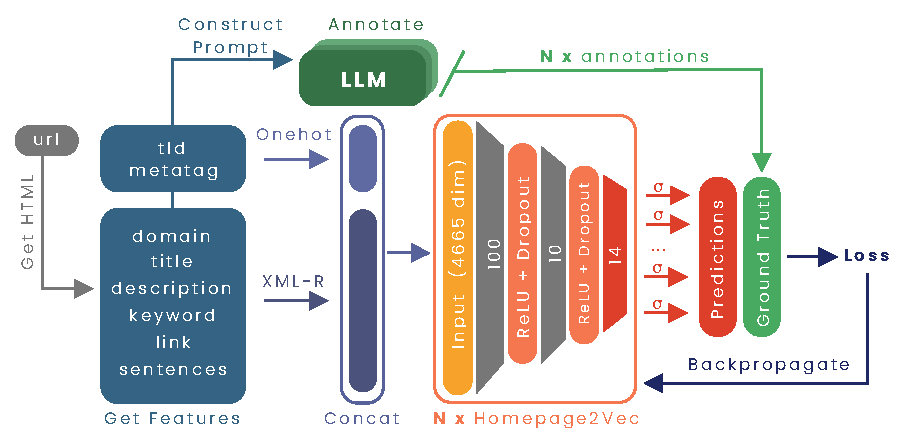
\includegraphics[height=0.2\textheight, width=\columnwidth]{./figures/training_overview.pdf}
    \caption{\textbf{Training overview.} Sth else}
    \label{fig:train-overview}
\end{figure}

Homepage2Vec, evaluated against an unbalanced Curlie test set, achieves a macro-averaged precision of $0.771$, recall of $0.549$, and an F1-score of $0.634$ \cite{homepage2vec}. While these results are promising, it is crucial to note that the majority of websites have at most one label. Therefore, the task is inherently easier than the one being addressed. To account for this, we evaluate the model on a crowdsourced dataset of 840 samples, where each website has an average of $2.5$ labels. We obtain a macro F1-score of $0.38$, serving as our baseline for further improvement using the proposed methods described in the following section.

% - GPT annotations 
\textbf{GPT-Based Labeling:} Utilizing GPT for streamlined annotation proves to be a powerful approach, as demonstrated in prior research \cite{reduce-labeling-cost, prompt-tuning, is-gpt3-good-annot, annollm}. While GPT-based labeling offers numerous advantages, relying on it for inference is suboptimal due to cost and time constraints, as suggested in previous work \cite{reduce-labeling-cost, is-gpt3-good-annot}. Instead, a more viable option is to employ GPT-generated labels for training a classifier, as pursued in this work. Additionally, our research extends beyond previous focuses on GPT-3, exploring the efficacy of GPT-4 for the same task. Finally, in contrast to prior studies, which focused solely on single-label classification with a limited number of classes \cite{reduce-labeling-cost, is-gpt3-good-annot}, our research expands the scope by investigating the effectiveness of GPT for multi-label classification tasks with $14$ possible classes.

\section{Methodology}\label{sec:methods}

% Mention the overall goal of our work to keep the big picture in mind
The overall goal of our work is to improve mutlilabel classification performance of the original homepage2vec model \cite{homepage2vec}. 
We refer to this model as \texttt{baseline}. 
We can divide our work into two main phases: (1) obtaining high-quality annotations and (2) fine-tuning the baseline model with the obtained annotations. 
In the following, we describe the methodology for each phase in detail.

\subsection* {Phase 1: Obtaining High-Quality Annotations}
In the first phase, we aim to obtion hight-quality GPT annotations measuring performance against human annotatated data.
The orignal human labaled data comprises of 840 websites, anotated each by 3 diffrent annotators. 
The measured inter-anotator agreement measured by the pairwise Cohen's kappa \cite{cohen-coef} is $0.2 \pm 0.02$, indicating low agreement. 
We assign a category label if at least 2 annotators agree, resulting in an average of $2.5$ labels per website.

For 761 websites that were reachable at the time of writing we scraped their content, extracting features such as top-level domain, domain, title, description, keywords, first 50 links, and first 100 sentences, the same features used in the original Homepage2vec model \cite{homepage2vec} and we used the same pipiline for feature embedding.
Also not all features were available for all websites, as shown in Table \ref{tab:feature_information}.
\begin{table}[!ht]
\centering
\caption{Percentage of websites with each feature accross our datasets.}
\label{tab:feature_information}
\begin{tabular}{lrr}
\toprule
 & Original & Curlie-gpt-10k \\
\midrule
n & 761.00 & 9190.00 \\
tld (\%) & 100.00 & 100.00 \\
domain (\%) & 100.00 & 100.00 \\
tags (\%) & 93.69 & 95.47 \\
titles (\%) & 98.42 & 98.28 \\
descriptions (\%) & 54.93 & 62.95 \\
keywords (\%) & 19.58 & 27.29 \\
links (\%) & 89.88 & 91.62 \\
sentences (\%) & 99.08 & 99.03 \\
\bottomrule
\end{tabular}
\end{table}


This scraped pre-prcessed data is then used to obtain the annotaions using Open-AI API.
The system prompt tells the model to perform a mutlilabel classification (the full prompr can be found in the Appendix \ref{app:prompt}) and to respod in a JSON format with key value pairs representing the category and the binary classification. Additionaly one example can website with the correct label is provided to the model, making it a texttt{1-shot} classificaion.
In the user promept we provided a JSON of the exctrated features, we considered 3 different contexts given to the model, accrding to features important found in the original paper \cite{homepage2vec}. 
The smallest context \texttt{context1} includes the least amount of information about the website, making the classification faster and cheaper as less tokens are used and the \texttt{context3} having all the information about the website that was scraped.

We also considered two versions of the GPT model an older GPT-3.5 model and a newer GPT-4 model, where the GPT-4 model is more expensive and slower to use.
All variants of the Labelers can be found in Tabel \ref{tab:labelers_setup}
% - introduce labelers (parameter dimensions), introduce prompt, one shot example:
\begin{table}[htbp]
    \centering
    \begin{tabular}{lll}
        \toprule
        \textbf{Parameter} & \textbf{Variants} & \textbf{Description} \\
        \midrule
        \texttt{context} 
            & \texttt{context1} & Uses the \texttt{tld}, \texttt{domain}, and \texttt{metatags} \\
            
            & \texttt{context2} & Same as \texttt{context1} plus \texttt{title}, \\ & & \texttt{description} and \texttt{keywords} \\
            
            & \texttt{context3} & Same as \texttt{context2} plus \texttt{links} and \\ & & \texttt{text}\\

        \addlinespace
        \texttt{model} 
            & \texttt{gpt3.5} & Uses GPT-3.5 (\texttt{gpt-3.5-turbo-1106}) \\
            
            & \texttt{gpt4}   & Uses GPT-4 (\texttt{gpt-4-1106-preview}) \\
        
        \addlinespace
        \texttt{fewshot} 
            & \texttt{fewshot} & Injects an example website and label into \\ & & the system prompt \\
            
            & \texttt{zeroshot} & Does not inject any example website or \\ & & label into  the system prompt \\
        \bottomrule
    \end{tabular}
    \caption{Description of Parameters and Variants}
    \label{tab:parameters}
\end{table}

\textbf{Curlie-10k} 
We employ the best-performing GPT annotator evaluated against the human annotated original crowdsourced data to annotate \texttt{curlie-10k}, a dataset with 10k randomly selected websites from Curlie. 
Following the same preprocessing and feature extraction as the original dataset, Table \ref{tab:feature_information} displays feature percentages across datasets. 
As the figure clearly indicates, the most useful features according to the homepage2vec \cite{homepage2vec} descriptions and keywords are missing in around 55 \% and 75 \% of cases, respectively. 

\begin{figure}[!ht]
    \centering
    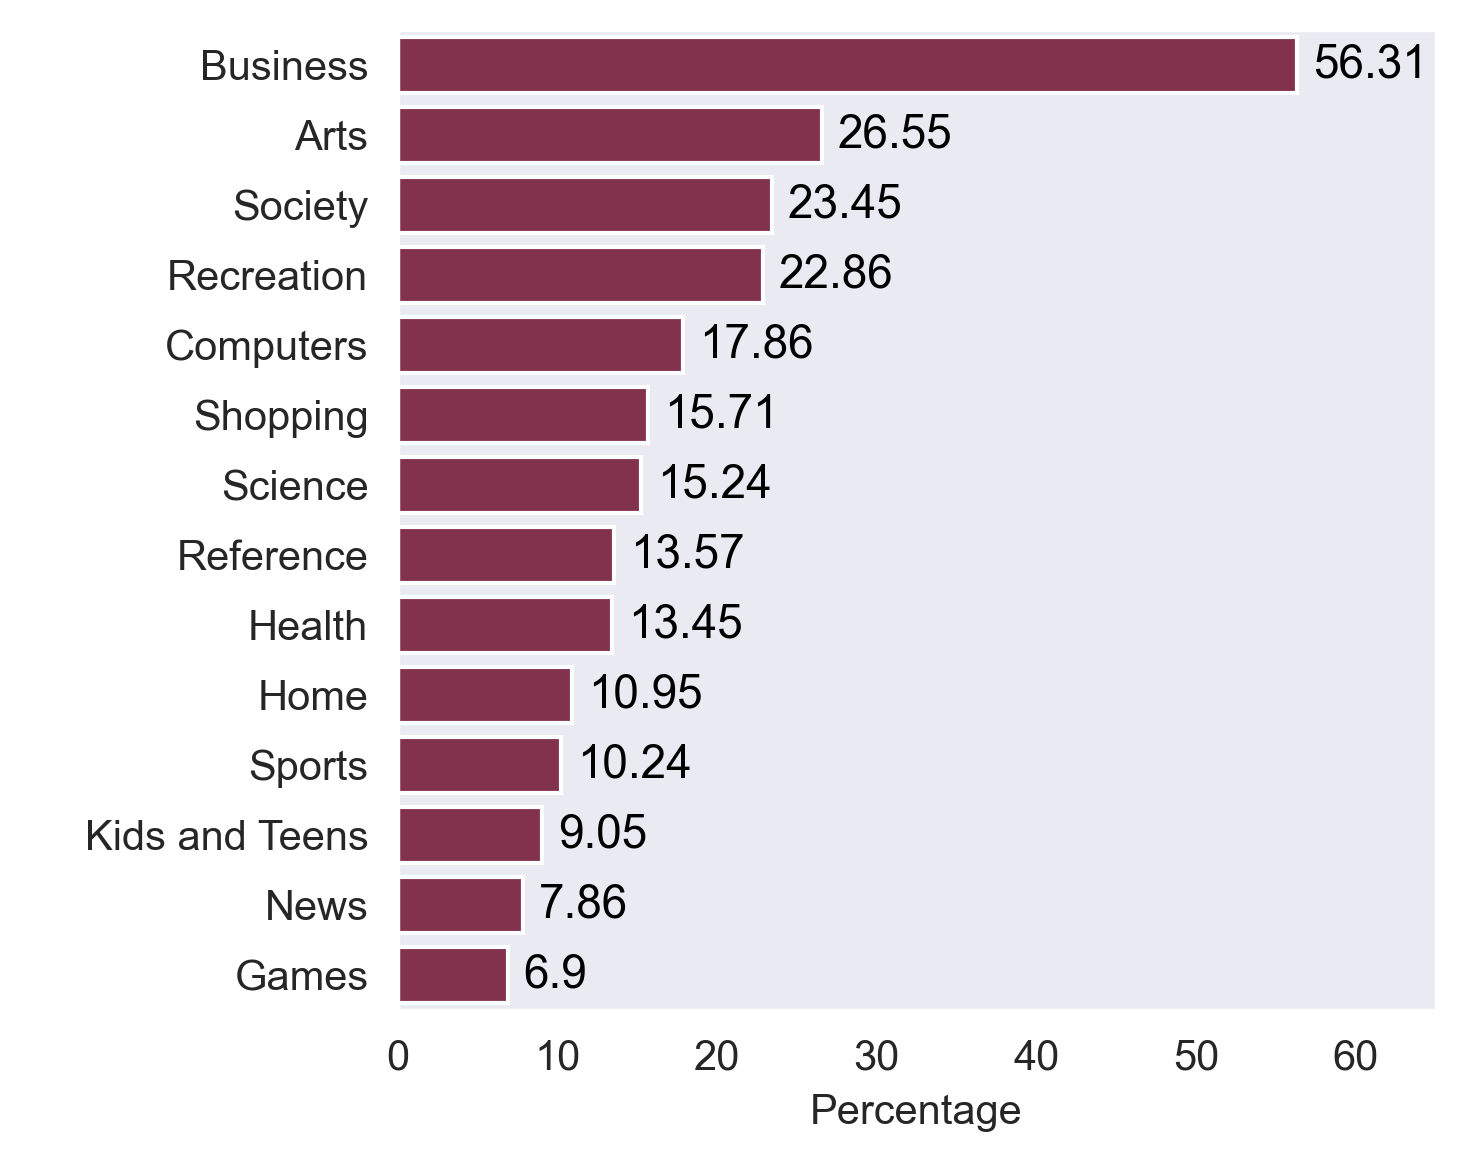
\includegraphics[width=1\columnwidth]{figures/category_distribution.png}
    \caption{Class distribution of the original dataset.}
    \label{fig:class_distribution}
\end{figure}

Figure \ref{fig:class_distribution} illustrates the class distribution of the original dataset. It is imbalanced, with most websites falling into the \textit{Business} category, followed by \textit{Arts} and \textit{Society}. This imbalance, identified in Homepage2vec, negatively impacted model performance on minority classes.
% 1. Step: Show that we can create high-quality annotations (measured against human annotations)
% - introduce curlie (talk about features (missing values), embedding, label list_ , re-scrape + process + embeddin
% ---> All this is pretty much in data, so transfer it here


% 2. Step: Show that we can improve performance compared to pre-trained model via fine-tuning with GPT annotations
% - training parameters (hparams, train/ test data splits)
% - evaluation procedure (macro f1, …)
% - calibration (?)
% TODO: this
\subsection* {Phase 2: Fine-Tuning the Baseline Model}
In the second phase, we fine-tune the baseline model with the obtained annotations from the \texttt{curlie-10k} dataset. And using the crowdsourced data as the test and validation set with 0.7/0.3 split.
We also perform a hyperparmeter search to find the best hyperparameters for the fine-tuning process. 
For this we employ Baeysian TPE samplerer from Optuna \cite{optuna} to efectively search the hyperparam space. 
The hyperparam values are detailed in Table \ref{tab:hyperparameters}.
\begin{table}[!ht]
    \centering
    \caption{\textbf{Hyperparameter Search Space}}
    \label{tab:hyperparameters}
    \begin{tabular}{ll}
    \toprule
    \textbf{Hyperparameter} & \textbf{Search Space} \\
    \midrule
    Learning Rate (\( \lambda \)) & $[0.00001, 0.01]$ \\
    Weight Decay (\( \beta \)) & $[0, 0.1]$ \\
    Scheduler Factor (\(\gamma\)) & $[0.1, 0.5]$ \\
    Batch Size (\(\delta\)) & \{64, 128, 256\} \\
    \bottomrule
    \end{tabular}
\end{table}


The best performing model is chosen by performance on the validation set using the multi-label macro F1 score, which is the average of the F1 score of each class. 
This model is then evaluated on the held out test set using macro F1, precision, recall, and accuracy.




\section{Results}

\subsection*{Phase 1: LLM Labeling}

\begin{table}[!ht]
\centering
\caption{\textbf{Labeler Statistics}}
\label{tab:labeler-results}
\begin{tabular}{lllccc}
\toprule
 &  &  &  \textbf{LPP} & \textbf{Cost} & \textbf{M.-F1} \\
\textbf{Model} & \textbf{Context} & \textbf{Shot} & ($\mu\pm\sigma$) & (\$) & (\%) \\
\midrule
\multirow[c]{6}{*}{
    \rotatebox[origin=c]{90}{GPT-3.5}
    } & \multirow[c]{2}{*}{\texttt{context1}} & 0-shot & 0.39 ± 0.61 & \textbf{0.36} & 15.96 \\
 &  & 1-shot & 0.91 ± 0.95 & 0.48 & 23.26 \\
 & \multirow[c]{2}{*}{\texttt{context2}} & 0-shot & 1.39 ± 0.98 & 0.42 & 37.59 \\
 &  & 1-shot & 1.68 ± 1.15 & 0.63 & 38.69 \\
 & \multirow[c]{2}{*}{\texttt{context3}} & 0-shot & 1.57 ± 1.08 & 0.57 & 37.24 \\
 &  & 1-shot & 1.85 ± 1.24 & 0.80 & 37.70 \\
\midrule
\multirow[c]{6}{*}{
    \rotatebox[origin=c]{90}{GPT-4}
    } & \multirow[c]{2}{*}{\texttt{context1}} & 0-shot & 1.50 ± 0.93 & 4.68 & 35.55 \\
 &  & 1-shot & 1.83 ± 1.36 & 5.75 & 36.10 \\
 & \multirow[c]{2}{*}{\texttt{context2}} & 0-shot & 2.16 ± 1.03 & 5.26 & 45.39 \\
 &  & 1-shot & 2.49 ± 1.28 & 7.25 & 45.93 \\
 & \multirow[c]{2}{*}{\texttt{context3}} & 0-shot & 2.30 ± 1.11 & 6.68 & 44.10 \\
 &  & 1-shot & 2.80 ± 1.30 & 8.99 & \textbf{46.12} \\
\bottomrule
\end{tabular}
\end{table}


Table~\ref{tab:labeler-results} presents important statistics of the re-labelling of the original crowdsourced corpus of websites using the LLM labelers introduced in Section \ref{sec:methods}.

% General Results: Consistency, Cost, Quality
\textbf{Results.} Our findings demonstrate that LLM labelers can provide \textit{consistent}, \textit{cost-effective}, and \textit{high-quality} annotations for the complex task of multi-lingual, multi-label website topic classification. 
Remarkably, not a single incorrect output was produced, underscoring the reliability and consistency of LLM-generated annotations.

In terms of cost, the labaling of the original crowdsourced corpus cost \$327, approximately \$(check if it fits) per 1000 pages.
Our approach, utilising GPT-3.5 and GPT-4 labelers, drastically reduces this cost to an average of
% Update the average for gpt4
 \$0.60 and \$6.30, respectively, achieving a reduction by factors of 217x and 21x.

% Calculations
% Human annotator cost: 327 USD % Pages annotated: 840 * 3 = 2520
% Cost per 1k page: 1000 * 327 / 2520 = 130$

% GPT labler cost/1k pages:
% (0.36 + 0.48 + 0.42 + 0.63 + 0.57 + 0.80 + 5.26 + 7.25) / 8 = 2.6

% GPT-3.5 labler cost/1k pages:
% (0.36 + 0.48 + 0.42 + 0.63 + 0.57 + 0.80) / 6 = 0.6

% GPT-4 labler cost/1k pages:
% (5.26 + 7.25) / 2 = 6.3

% Cost reductions:
% GPT-3.5: 130 / 0.6 = 217x
% GPT-4: 130 / 6.3 = 21x

Performance-wise, GPT-4 labeler peaks at a 46\% macro F1 score using context 2 and 1-shot, outperforming the baseline of the pre-trained model. 
The improvements suggest that we can expect to improve the performance of the pre-trained model by fine-tuning it with the LLM labels if we can distil the knowledge from the LLMs into the pre-trained model - the goal of the second phase of our study.

% GPT labeler parameter grid
\textbf{Labeler Parameter Grid.} Figure~\ref{fig:labelers-grid} visualises the effect of the labeler parameters on the macro F1 score. As expected, we find that the quality of the labels increases with the amount of context provided and the quality of the model used. 
Interestingly, the added feature in the context3 (links and text) do not increase the annotation quality for the GPT-3.5, but do for the GPT-4. 
We hypothesize that this is due to the fact that the smaller model can get confused with the the additional features that are very long compared to the prompt, while the larger model can handle the additional features better. 


\begin{figure}[!h]
    \centering
    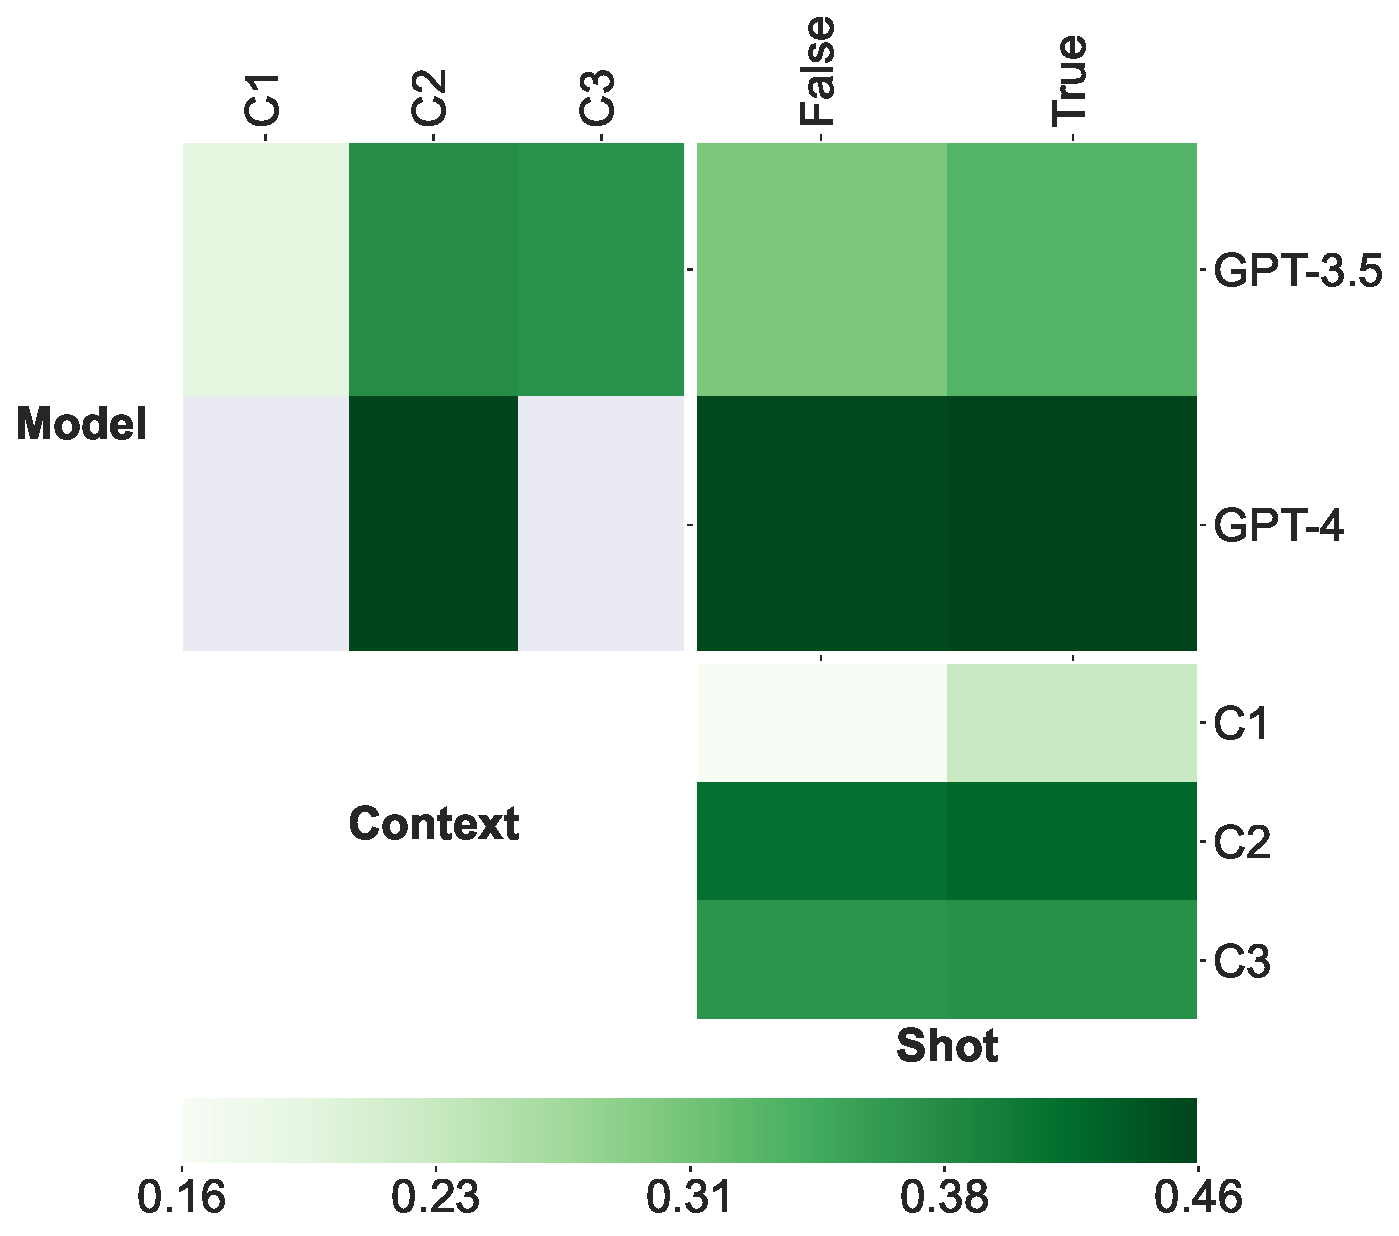
\includegraphics[width=.8\columnwidth]{./figures/labelers-grid.pdf}
    \caption{\textbf{Labeler Parameter Grid:} Macro F1 score for all combinations of the LLM labeler parameters.}

    \label{fig:labelers-grid}
\end{figure}

% Cost-quality trade-off
\textbf{Cost-Quality Trade-Off.} 
Out analysis reveals a positve trend between label quality and cost, attributable to the use of longer prompts or more sophisticated models.
The optimal compromise is achieved with a GPT-3.5 annotator utilizing context 2 and a few-shot example. This configuration ensures a robust label quality at 39\% (only a 15\% decrease) while cutting the cost per 1000 pages from \$7.25 to \$0.63 (a 91\% decrease). 
This GPT-3.5 annotator was used to label the texttt{curlie-gpt3.5-10k} dataset, which we use in the second phase of our study.

% Curlie-10k dataset
The average number of topics assigned to a page is \textbf{1.6}, which is higher than the average of \textbf{1.07} for the original Curlie dataset. 
Figure~\ref{fig:label-distribution-comparison} shows the distribution of the labels in the re-labelled dataset compared to the original Curlie dataset.
We observe that the number of labels increased for every class.

\begin{figure}[!h]
    \centering
    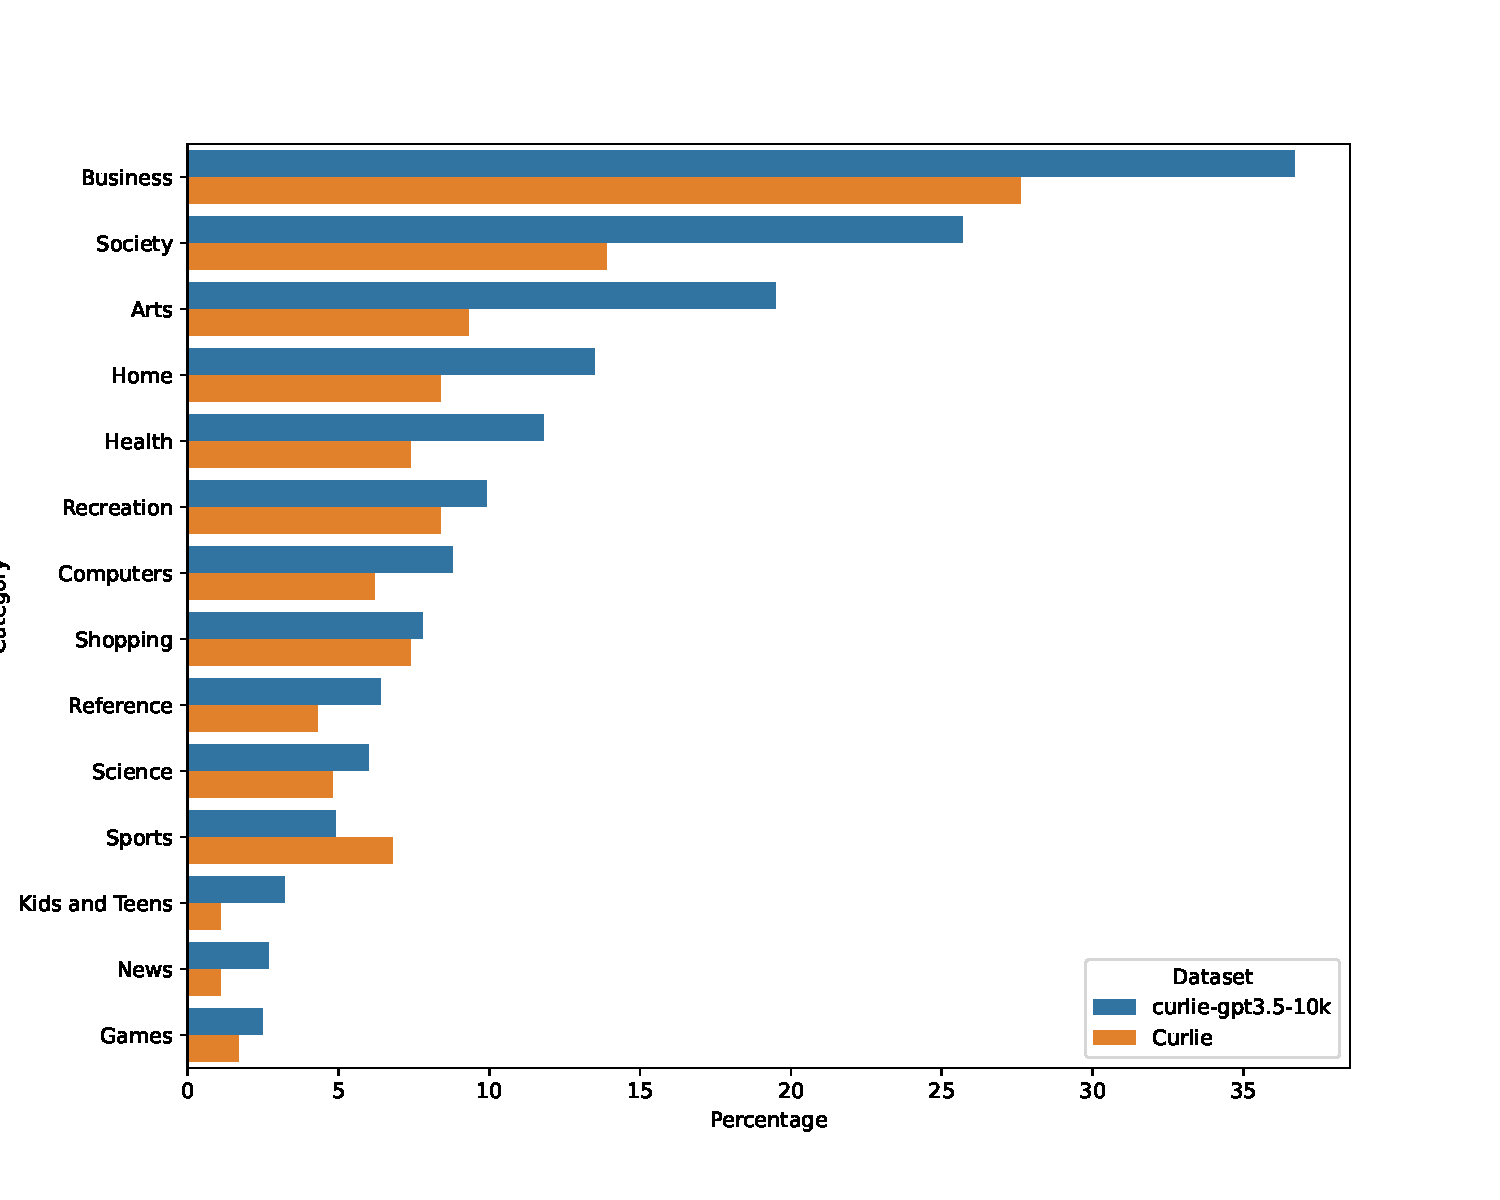
\includegraphics[width=.8\columnwidth]{./figures/class_distribution_comparison.pdf}
    \caption{\textbf{Curlie-10k Label Distributino.} We show the topic distribution of the Curlie-10k dataset.}
    \label{fig:label-distribution-comparison}
\end{figure}


\subsection*{Phase 2: Knowledge Distillation}

% TODO: Would be cool to compare the labelling statistics of the exact 10k subsplit (Curlie vs. GPT) -- for now we will proxy.

The goal of the second phase of the study is to transfer the knowledge from the LLMs into the pre-trained model. 
To this end, we use the \texttt{curlie-gpt3.5-10k} dataset for fine-tuning the pre-trained model.


% Fine-tuning results
\textbf{Finetuning.} Table~\ref{tab:finetune-results} shows the results of the fine-tuning experiment. 
We observe that the fine-tuned model increases the recall significantly from 39.4\% to 47.6\%, at the cost of a minor decrease in precision from 40.9\% to 40.2\%. 
This increases the overall macro F1 score from 39.2\% to 42.6\%, which is a 9\% improvement. 
We have shown that the approach of fine-tuning the pre-trained model with the LLM labels can improve the performance on the texttt{crowdsourced} dataset that better resembles the true website topic classification.

% 0.391610 = 39.2% (Pre-trained Homepage2Vec)
% 0.426289 = 42.6% (GPT-3.5)
% Absolute Difference: 0.034679 = 3.5 percentage points
% Relative Difference: 0.086 = 8.6%

\begin{table}[!ht]
\centering
\caption{\textbf{Finetuning Results.} The table shows the precision, recall, macro F1 and and labels per page when evaluated on \texttt{crowdsourced}. We show results for the pre-trained baseline, as well as both finetuned variants.}
\label{tab:finetune-results}
\begin{tabular}{lrrrr}
\toprule
 & \textbf{Pr.} & \textbf{Re.} & \textbf{M.-F1} & \textbf{LPP} \\
 & (\%) & (\%) & (\%) & ($\mu$) \\
\midrule
Pretrained & \textbf{40.97} & 39.44 & 39.16 & 1.84 \\
GPT-3.5 & 40.19 & 47.55 & 42.63 & 1.93 \\
GPT-4 & 39.92 & \textbf{49.07} & \textbf{42.87} & \textbf{3.07} \\
\bottomrule
\end{tabular}
\end{table}


Figure~\ref{fig:finetune-results} shows the class-wise F1 score for the pre-trained model and the fine-tuned model. We observe that the fine-tuned model consistently outperforms the pre-trained model, achieving higher F1 scores in ten out of the 14 classes.


\begin{figure*}
    \centering
    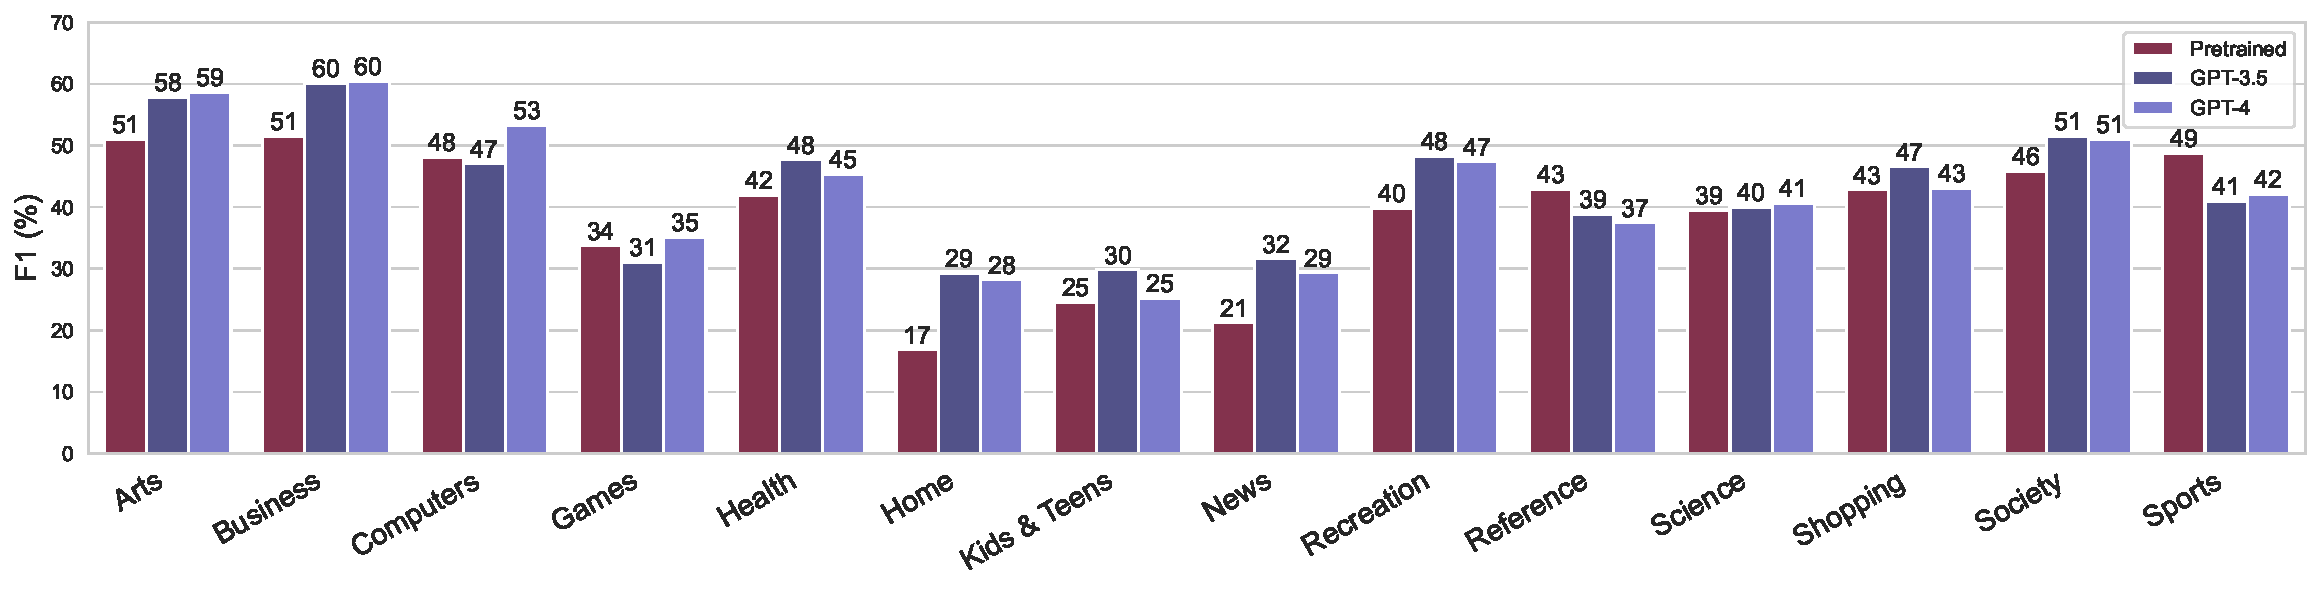
\includegraphics[width=\textwidth]{./figures/exp2-mf1.pdf}
    \caption{\textbf{Finetune Results.} Class-wise F1 score for the pre-trained model and the fine-tuned model on te original crowdsourced data.}
    \label{fig:finetune-results}
\end{figure*}


\newpage
\bibliographystyle{IEEEtran}
\bibliography{literature}


\appendix

\section{Additional Information}
\label{app:prompt}
This appendix details the GPT prompt used for website topic classification. 

\textbf{System Prompt:} 
\begin{quote}
    You are an expert in website topic classification that accurately predicts the topic. Analyze the provided website data and classify it into relevant categories.
\end{quote}

\begin{verbatim}
["Arts", "Business", "Computers", "Games", "Health", "Home", 
"Kids_and_Teens", "News", "Recreation", "Reference", "Science", 
"Shopping", "Society", "Sports"]
\end{verbatim}

\textbf{Output Format:}
\begin{quote}
    Output a JSON string with categories as keys and binary values (0 or 1) indicating if the webpage belongs to the topic. Always include all categories in the JSON output. If the labeler is one-shot, the example website is included in the JSON output as well.
\end{quote}

\textbf{Example provided if the model is \texttt{1-shot}:}
\begin{quote}
    Given website data: \\
    \begin{verbatim}
{         
    "title": "The New York Times ...",
    "description": "Find breaking news ...",
    "keywords": [
        "breaking news",
        "...",
    ],
    "links": [
        "breaking-news",
        "...",
    ],
    "tld": "com",
    "domain": "nytimes.com",
    "metatags": ["NYT", "..."],
    "sentences": [
        "Breaking news: A major political development reshapes the landscape in Washington.",
        "...",
    ]
}
        \end{verbatim}
    A good classification is:
    \begin{verbatim}
{
    "Arts": 1,
    "Business": 1,
    "Computers": 0,
    "Games": 0,
    "Health": 1,
    "Home": 0,
    "Kids_and_Teens": 0,
    "News": 1,
    "Recreation": 0,
    "Reference": 0,
    "Science": 1,
    "Shopping": 0,
    "Society": 1,
    "Sports": 1
}
    \end{verbatim}
\end{quote}


\end{document}


% Some important notes from the homepage2vec paper
% 1) Intro
% Before homepage2vec
% - No multilingual models
% - No embeddings based methods
% - Usually paid services
% With Homepage2vec
% - multilingual -> great because out of top 10M websites, 40% are not in English
% - embeddings based
% - open source
% - fast since you can run it locally, and do not have to use external API

% 2) Related work
% Related approaches
% - manual approaches back in the days
% - ML based methods that use contextual features of the given webpage
% - Methods that also use for context the surrounding webpages, especially useful when the current page does not include that much info
% - Methods that use vision features
% - Recently, use of the LSTM, BERT, GRU architectures -> shown to increase performance -> however focus purely on English

% Multilingual embeddings
% - They are using XML-R, multi-lingual model, that has shown to be comparable to the monolingual models

% 3) Dataset
% - Curlie = community edited web directory -> 3M websites in 92 languages,
% labeled in hierarchical categories, however they only used the top level categories
% Originally, there were 15 top level categories, but they dropped "Regional"
% - Majority of classes associated with Bussiness (27), Society (13.9) or Arts (9)
% - 40% of the websites are in English, 16 % in German, 5% in french, 6% in Japanese
% - Although each page may, in principle, have an arbitrary number of category labels, 
% at the top level, the data is mostly single-labeled, with only 2.1% of samples appearing 
% in two or more taxonomy trees of the 14 top-level classes.

% 4) Method
% - They embeded only the first 100 sentences since the embedding process is quite expensive
% This was selected based on the validation set performance using the elbow method
% - They use 19 most frequent domains exluding the domains that indicate country
% - Title, description and keywords are used as well and should be very informative
% - With the links, they use the anchor text and the 50 most frequent texts are used, again
% this was selected using the elbow method

